\section{Microservice-Architekturen und Sicherheit}

Ein Microservice-basiertes System ist ein verteiltes System, das in der Regel auf mehreren Maschinen läuft. Auf jeder dieser Maschine laufen ein oder mehrere Microservices. Dabei dürfen Services sich während des Ausführungszeit nicht gegenseitig beeinflussen. Viele Teile des Systems müssen kommunizieren, entweder es werden Nachrichten bzw. Tasks entgegen genommen oder Nachrichten verschickt \cite{newman2015}. Ein breiter Angriffsvektor entsteht.

Dieses Kapitel beschreibt zunächst gängige Technologien zum Bau von Microservices und geht auf Sicherheit im Sinne von Isolation ein. Anschließend werden Möglichkeiten betrachtet, koplexe Systeme auf Microservice-Basis zu ermöglichen. Die dabei entstehenden architekturellen Herausforderungen sowie auch mögliche Sicherheitsprobleme werden hervorgehoben. Mögliche Ansätze zum Schutz eines Microservice-basierten Systems werden diskutiert.


\subsection{Technologien zum Bau von Microservices}

Ein Microservice sollte replizierbar (und somit skalierbar), sowie einfach zu deployen und sicher sein \cite{newman2015,microservicesIO}. Um Skalierbarkeit und einfaches Deployment zu erreichen, bietet es sich wiederum an Microservices in ähnlichen Ausführungsumgebungen laufen zu lassen. Das jedoch steht im Wiederspruch zu dem Konzept der Service-Unabhängigkeit und Autonomie. 

\subsubsection{Virtuelle Maschinen}
Mit herkömmlichen Virtualisierungstechnologien, wie etwa VMWare lässt sich die gewünschte Abstraktion schaffen. Services werden als Images für die virtuelle Maschine (\textit{VM}) spezifiziert und können somit repliziert und portiert werden. Auch das Deployment des Services ist dann einfacher, weil nur noch das Service Image in der entsprechenden virtuellen Maschine gestartet werden muss.

Wenn mehrere Microservices den gleichen Host oder die gleiche VM teilen, sind sie nicht unabhängig \cite{microservicesIO}. Bei böswilliger Manipulation oder Infiltrierung eines Services könnten auch andere Services im gleichen System beeinflusst werden. Folgt man dem Konzept so wäre es korrekt und sicher(-er) einen Service pro Host oder VM zu deployen. Das resultiert allerdings in Resourcen-Overhead der benötigt wird, um die (möglicherweise vielen) virtuellen Maschinen bzw. Hosts zu betreiben \cite{newman2015}. Die Grafik \ref{fig:container-vm} zeigt die Resourcen auf, die bei einem Setup mit virtuellen Maschinen benötigt werden und zeigt vergleichsweise den Resourcen-Verbrauch eines Container-basierten Setups.

Der Ansatz, ein Microservice-basiertes System mit virtuellen Maschinen zu realisieren bringt jedoch auch Sicherheitsvorteile mit sich. Sofern wirklich nur ein Service pro virtueller Maschine läuft, sind alle Services des Systems vollständig unabhängig voneinander. Somit ist das Gesamtystem weniger Anfällig für Ausfälle oder bösartige Manipulation einzelner Services.

\begin{figure}[h]
    \centering
    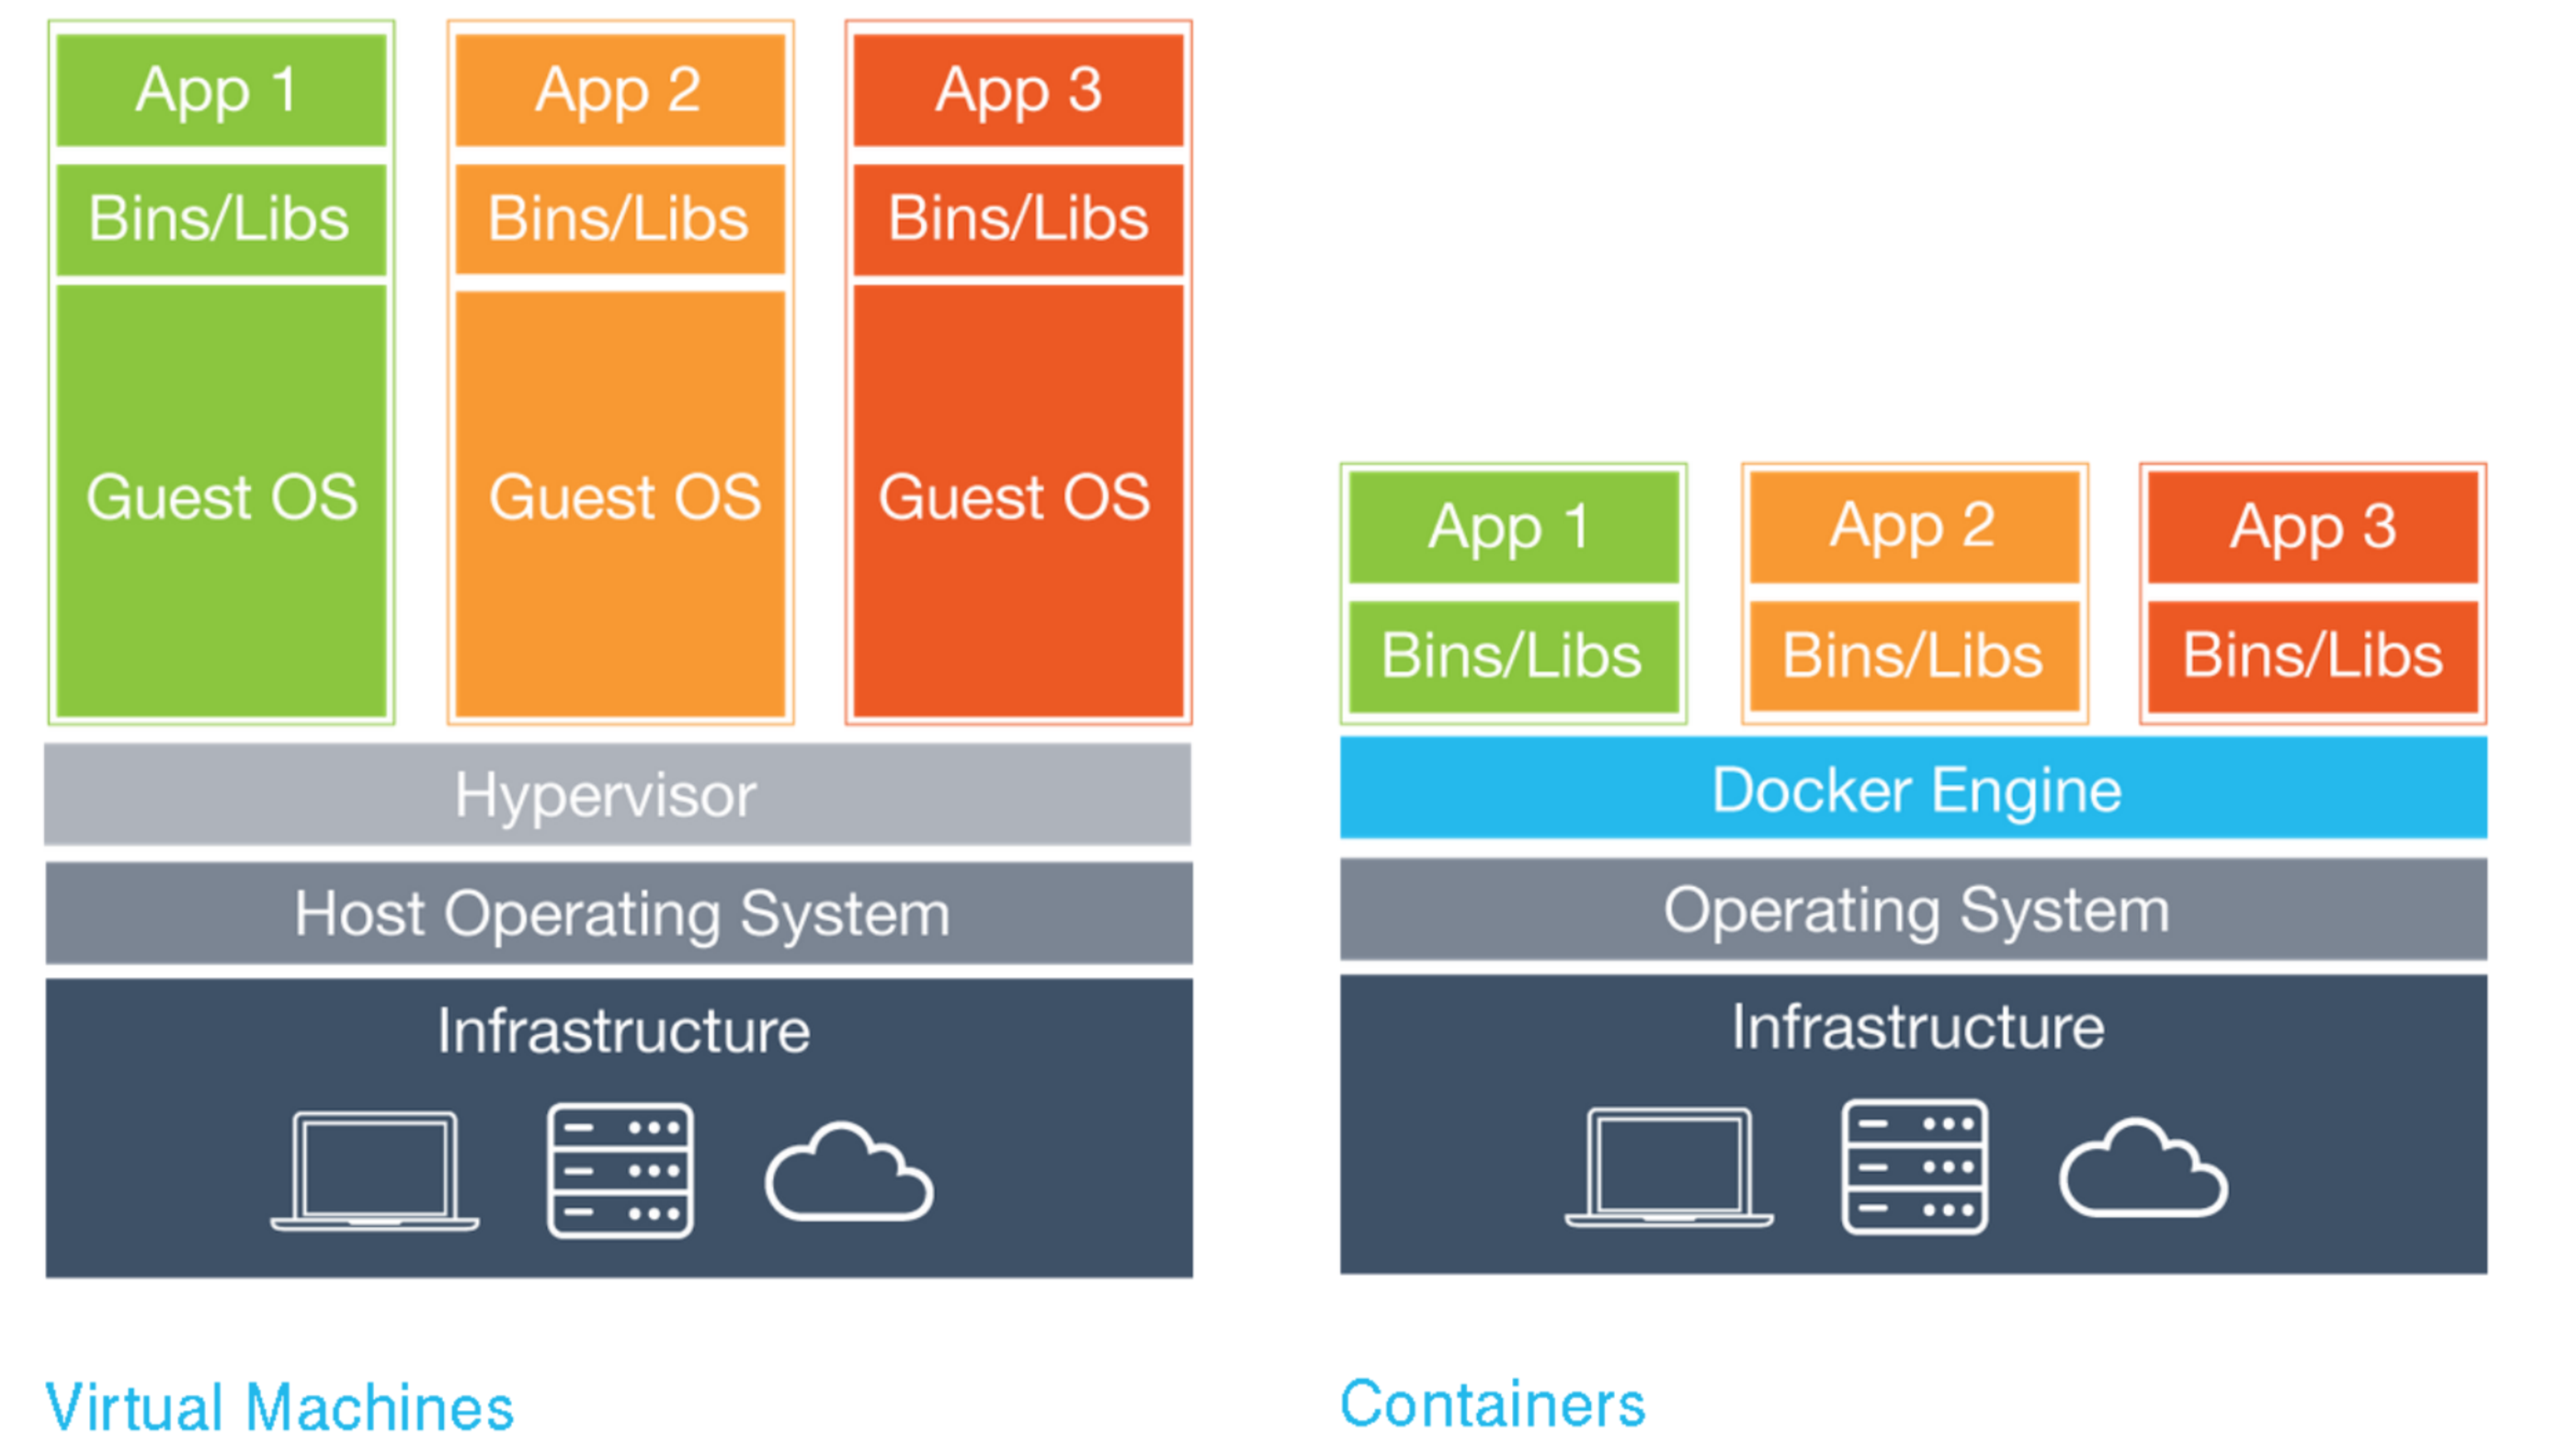
\includegraphics[scale=0.3]{img/container-vm.pdf}
    \caption{Vergleich von standard Virtualisierung und Docker Conainern, entnommen von \url{http://www.docker.com/what-docker}}
    \label{fig:container-vm}
\end{figure}

\subsubsection{Container}
Ein Container ist ein schlanker „Wrapper“ um einen Linux Prozess. Wir betrachten hier \textit{Docker}\footnote{\url{https://www.docker.com}} als Container Engine, es sei aber noch LXC (Linux Containers) erwähnt.

Docker und Docker-Container bieten ähnliche Funktionen wie eine virtuelle Maschine und zugehörige VM Images. Allerdings sind Container um ein Vielfaches leichtgewichtiger als VMs. Während eine VM ein Gast-Betriebssystem und eigene Bibliotheken enthält, enthalten Container nur eine Anwendung und deren benötigte Abhängigkeiten. Container teilen sich den Kernel des ausführenden Host-Betriebssystems und laufen als einzelner Prozess im Userland \cite{newman2015}. Die Grafik \ref{fig:container-vm} zeigt deutlich, auf welche Weise Container leichtgewichtiger sind als virtuelle Maschinen.

Zusätzlich werden Container durch Container Images spezifiziert -- genauso wie bei VMs -- was die Vervielfältigung ungeheuer einfach macht. Allerdings ist die Modifikation von Dockerimages einfacher als das Ändern eines VM Images. Docker ermöglicht mithilfe eines sogenannten \textit{Dockerfile}s sehr einfache Manipulation von Images. 
Docker bietet hervorragende Sicherheit im Sinne von Isolation. Durch die intelligente Verwendung von \textit{Namespaces}, \textit{Network Interfaces} und \textit{Cgroups} werden in Containern laufende Prozesse vollständig von anderen Prozessen des ausführenden Systems isoliert \cite{newman2015,marmol2015}. Laufende Docker Container haben einen eigenen Namespace. Für Prozesse innerhalb des Containers sind jegliche andere Prozesse nicht sichtbar und nicht beeinflussbar -- ob auf dem ausführenden Host-Betriebssystem oder in anderen Containern. Jeder Container hat einen eigenen Network-Stack, wodurch jeder Container nur Einfluss auf seinen eigenen Traffic nehmen kann. Zuletzt wird der Resourcenverbrauch reguliert durch Control Groups, ebenfalls ein Linux Kernel Feature. Es wird garantiert, dass ein Container genügend Resourcen bekommt, um zu arbeiten; es kann auch eingeschränkt werden, dass ein Container nicht zu viele Resourcen des Host-Betriebssystems verbraucht\footnote{Detaillierte Informationen zu Docker Security: \url{https://docs.docker.com/engine/articles/security/}}.

Dockers Charakteristika legen nahe, wie gut diese Technologie geeignet ist um die Anforderungen abzudecken, die eine Microservice-Architektur mit sich bringt. Durch das Design von Docker sind in Containern laufende Prozesse vollständig unabhängig voneinander. Services lassen sich in Form von Images einfach replizieren und portieren. Das ausführende System ist unwichtig, solange es ein Linux System ist und Docker installiert ist. Zum Thema Microservices, die mit Hilfe von Docker realisiert werden finden sich viele aktuelle Softwareprojekte.


\subsection{Managing Microservices / Orchestrierung}

Es gibt verschiedene Möglichkeiten, Microservices mit einander interagieren zu lassen um daraus ein komplexeres System entstehen zu lassen. Generell gilt für Microservices, dass sie \textit{klein}, auf \textit{eine Aufgabe} spezialisiert und \textit{autonom} sind \cite{newman2015}. Das bedeutet insbesondere auch, dass Services eines Systems einander meist nicht kennen. Im Folgenden werden einige Herausforderungen diskutiert, die beim Bau eines Microservice-basierten Systems entstehen. Es werden Software Lösungen und Frameworks vorgestellt, die viele der Problemstellungen intelligent lösen. Sicherheitskritische Bereiche werden aufgezeigt und Maßnahmen zu deren Schutz erläutert. Anschließend wird das opensource Project \textit{Kubernetes} von Google vorgestellt.

\subsubsection{Systemanforderungen}

Bei einem System aus autonomen Microservices muss auch das Deployment der Services autonom sein. Services zu starten/stoppen, zu verändern oder zu verfielfätigen sollte vom Gesamtsystem ermöglicht werden, während andere Services davon nicht beeinflusst werden. Das Gesamtsystem muss den Ausfall einzelner Services verkraften. Für Entwickler oder Administratoren muss ersichtlich sein, welche Komponenten des Systems korrekt oder inkorrekt arbeiten \cite{newman2015}. Aus diesen Anforderungen und aus der Spezifikation von Microservices \todo{ref auf kap 1} ergeben sich einige problematische Fragestellungen, die gelöst werden müssen.

Wenn Services autonom agieren und einzeln an- und abschaltbar sind, wie können sie dann miteinander kommunizieren? Microservices haben in der Regel keine feste IP Adresse, unter der sie immer erreichbar sind. Dieses Problem wird als \textit{Service Discovery} bezeichnet. Services müssen einander im System finden, um Nachrichten austauschen zu können. Technisch lässt sich das Problem beispielsweise durch den Einsatz einer DNS (Domain-Name-System) lösen. Auch \textit{etcd}\footnote{\url{https://coreos.com/etcd/docs/latest/}} ließe sich dafür verwenden.

Wie lässt sich das Verhalten einzelner Services nachvollziehen? Dazu kann zentralisiertes Logging verwendet werden; alle Microservices schicken ihre Logs zu einem Service, der allein dafür zuständig ist, Lognachrichten zu akkumulieren. Ein sehr häufiges Setup ist der sogenannte \textit{ELK-Stack}\footnote{\url{https://www.elastic.co/webinars/introduction-elk-stack}}. Dabei wird \textit{Logstash} als zentralisierter Log-Akkumulator verwendet, die Logs werden anschließend in einer \textit{Elasticsearch} gespeichert und mit \textit{Kibana} visualisiert. Ebenfalls populär, insbesondere im Container Umfeld sind \textit{InfluxDB}\footnote{\url{https://influxdb.com/}} und \textit{Grafana}\footnote{\url{http://grafana.org/}} womit sich Zeitbasiert Metriken gut visualisieren lassen.

Das Sichten von Lognachrichten erfordert in der Regel menschliche Interaktion und nur mit Logging lässt sich nicht gezielt abfragen, ob ein Service überhaupt arbeitet oder nicht. Daher werden \textit{Healthchecks} für jeden einzelnen Microservice benötigt. Ein Healthcheck gibt Auskunft darüber, ob ein Service läuft und arbeitsfähig ist. Für jeden Microservice kann ein Healthcheck unterschiedlich sein, beispielsweise ein einfacher Ping für einen Rest-Service oder ein Select-Statement für eine Datenbank.

Wie lässt sich das System skalieren? Da die Microservices des Systems einfach replizierbar und portierbar sind, kann bei hoher Last auf einem Service einfach weitere Services hinzugefügt werden, die die selbe Aufgabe erfüllen. Man spricht von horizontaler Skalierung. Damit dies jedoch fehlerfrei funktionieren kann, muss Service Discovery (s.o) und auch Loadbalancing im System vorhanden sein.

Wenn mehrere Services die gleiche Aufgabe übernehmen, muss das Gesamtsystem entscheiden, welcher Service welche Aufgaben erhält. Das nennt man Loadbalancing. Gleiche Arbeit wird von replizierten Services übernommen, aber wie kann entschieden werden, welcher Service gerade bereit für neue Last ist? Hier können simple Verfahren wie etwa Round-Robin eingesetzt werden; häufig werden jedoch erprobte Systeme wie etwa \textit{HAProxy}\footnote{\url{http://www.haproxy.org/}} oder \textit{Nginx}\footnote{\url{http://nginx.org/}} verwendet.

Zuletzt bleibt noch die Frage nach Sicherheit. Zum einen muss die Kommunikation zwischen den Services sicher sein, Nachrichten dürfen nicht manipuliert werden. Klassische Angriffsszenarien wie beipielsweise ein Man-In-The-Middle Angriff zwischen Services sollte nicht möglich sein. Zum anderen muss auch das gesamte System gesichert sein. Die Ausführung, das Deployment oder Balancing von Services darf für Unbefugte nicht manipulierbar sein. 

Im Folgenden stellen wir kurz das Open-Source-Projekt \textit{Kubernetes} vor. Es wird diskutiert, wie das System in seiner Gesamtheit vor unbefugtem Zugriff geschützt wird. Auf die „Servicekommunikation und Sicherheit“ gehen wir dann im darauf folgenden Kapitel detaillierter ein.

\subsubsection{Kubernetes}
Es gibt viel Bewegung im Feld um Microservices und Docker. Viele großangelegte Projekte, getrieben durch führende Software-Konzerne\footnote{Kubernetes//Google: \url{http://kubernetes.io}, Mesos//Apache: \url{http://mesos.apache.org}, Azure//Microsoft: \url{http://azure.microsoft.com}, ECS//Amazon: \url{https://aws.amazon.com/de/ecs/}} nehmen maßgeblich Einfluss auf die Softwareentwicklung in diesem Gebiet. Kubernetes, eines dieser Projekte ist eine opensource Software, gestartet von Google und wird von einer wachsenden Community weiter vorangebracht.
